\section{Ensembles e bagging}\label{sec:bagging}

\begin{frame}{A sabedoria das multidões}
\begin{itemize}
  \item Faça uma pergunta difícil a milhares de pessoas e agregue as respostas. Em geral, a resposta agregada é \alert{melhor} que a de um único especialista: é a \emph{sabedoria das multidões}.
  \item Mesma ideia em aprendizado de máquina: agregue as previsões de um \alert{grupo de preditores}. O resultado costuma ser melhor que o do melhor preditor individual.
  \item Um grupo de preditores é um \alert{ensemble}, e o algoritmo que o constrói é um \alert{método de ensemble}.
  \item Por que interessa a árvores? Uma árvore é \alert{instável} (alta variância); combinar muitas pode compensar isso.
\end{itemize}
\vspace{4pt}
\centering
\begin{tikzpicture}[
  caixa/.style={draw,rounded corners=2pt,minimum height=0.6cm,inner sep=3pt,font=\small},
  seta/.style={-{Latex[length=1.8mm]}}]
\node[caixa] (x) at (0,0) {$\mathbf x$};
\node[caixa] (h1) at (3,0.9) {$h_1(\mathbf x)$};
\node[caixa] (h2) at (3,0) {$h_2(\mathbf x)$};
\node at (3,-0.55) {$\vdots$};
\node[caixa] (hB) at (3,-1.2) {$h_B(\mathbf x)$};
\node[caixa,fill=blue!8] (ag) at (6.4,0) {agregação};
\node[caixa] (y) at (9,0) {$\hat y(\mathbf x)$};
\foreach \h in {h1,h2,hB}{\draw[seta] (x) -- (\h); \draw[seta] (\h) -- (ag);}
\draw[seta] (ag) -- (y);
\end{tikzpicture}

% [MANIM] a multidão de preditores votando
\end{frame}

\begin{frame}{Votação por maioria (\emph{hard voting})}
Sejam $h_1,\dots,h_B:\R^p\to\{1,\dots,K\}$ classificadores treinados. O \alert{classificador por votação} devolve a classe mais votada (a moda):
\[
\hat y(\mathbf x)=\argmax_{k}\ \sum_{b=1}^{B}\ind\bigl(h_b(\mathbf x)=k\bigr).
\]
\begin{itemize}
  \item Exemplo com $B=3$: votos $1,0,1\ \Rightarrow\ \hat y=1$.
  \item Surpresa: o ensemble pode superar \alert{até o melhor} membro, mesmo que cada membro seja individualmente fraco.
  \item Quando isso acontece? Veja o próximo slide.
\end{itemize}
\end{frame}

\begin{frame}{Por que funciona: lei dos grandes números}
\begin{columns}[T]
\column{0.47\textwidth}
\small
Suponha $B$ classificadores \alert{independentes}, cada um correto com probabilidade $p>\tfrac12$. O número de acertos é $X\sim\mathrm{Binomial}(B,p)$ e a maioria acerta se $X>B/2$:
\[
P(\text{maioria correta})=\sum_{k>B/2}\binom Bk p^k(1-p)^{B-k}.
\]
\begin{itemize}
  \item Pela lei dos grandes números, $X/B\to p>\tfrac12$, e portanto a probabilidade $\to1$ quando $B\to\infty$.
  \item Cota de Hoeffding: $\ \ge 1-e^{-2B(p-1/2)^2}$.
\end{itemize}
\column{0.52\textwidth}
\centering
\begin{tikzpicture}
\begin{axis}[width=\linewidth,height=5.6cm,xmode=log,
  xlabel={número de classificadores $B$},ylabel={$P(\text{maioria correta})$},
  ymin=0.45,ymax=1.03,ymajorgrids,grid style={gray!25},
  tick label style={font=\scriptsize},label style={font=\small},
  legend style={font=\scriptsize,at={(0.97,0.05)},anchor=south east,draw=none,fill=none}]
\addplot[thick,color={rgb,255:red,127;green,179;blue,232}] table[x=B,y=p51]{../python/ensembles/figures/maioria.dat};
\addplot[thick,color={rgb,255:red,42;green,120;blue,214}] table[x=B,y=p55]{../python/ensembles/figures/maioria.dat};
\addplot[thick,color={rgb,255:red,20;green,74;blue,143}] table[x=B,y=p60]{../python/ensembles/figures/maioria.dat};
\legend{$p=0{,}51$,$p=0{,}55$,$p=0{,}60$}
\end{axis}
\end{tikzpicture}
\end{columns}
\end{frame}

\begin{frame}[fragile]{Números: votos independentes}
\lstinputlisting[style=py,basicstyle=\ttfamily\footnotesize]{../python/ensembles/01_maioria.py}
\vspace{4pt}
{\footnotesize\textbf{Saída}}
\lstinputlisting[style=saida,basicstyle=\ttfamily\footnotesize]{../python/ensembles/outputs/01_maioria.txt}
\vspace{2pt}
\begin{itemize}
  \item Mesmo com $p=0{,}51$ (quase uma moeda), $B=10\,000$ votos dão $\approx97{,}7\%$ de chance de a maioria acertar.
\end{itemize}
\end{frame}

\begin{frame}{Atenção: a premissa é a independência}
\begin{itemize}
  \item Classificadores treinados nos \alert{mesmos dados}, com o mesmo algoritmo, tendem a cometer os \alert{mesmos erros}. Se erram juntos, a maioria erra junto.
  \item Exemplo: $B=3$ classificadores com acurácia $p=0{,}70$.
  \begin{itemize}
    \item independentes: $P(\text{maioria correta})=3p^2-2p^3=0{,}784$;
    \item idênticos: $0{,}700$ (a votação não ajuda).
  \end{itemize}
  \item Para ganhar com o ensemble é preciso \alert{diversidade}. Duas formas:
  \begin{enumerate}
    \item \alert{algoritmos diferentes} nos mesmos dados (votação);
    \item o \alert{mesmo algoritmo} em \alert{amostras diferentes} dos dados (bagging).
  \end{enumerate}
\end{itemize}
\end{frame}

\begin{frame}{Votação suave (\emph{soft voting})}
Se cada classificador estima probabilidades $\hat p_b(k\mid\mathbf x)$, podemos \alert{tirar a média} delas:
\[
\hat y(\mathbf x)=\argmax_{k}\ \frac1B\sum_{b=1}^{B}\hat p_b(k\mid\mathbf x).
\]
\begin{block}{Mini-exemplo ($B=3$, probabilidade da classe 1)}
$0{,}90,\ 0{,}45,\ 0{,}45$.\quad \textbf{Hard}: votos $1,0,0\Rightarrow$ classe $0$. \quad \textbf{Soft}: média $=0{,}60\Rightarrow$ classe $1$.
\end{block}
\begin{itemize}
  \item Dá mais peso a votos \alert{confiantes}. Exige que os membros tenham \texttt{predict\_proba}.
  \item A documentação do scikit-learn a recomenda para classificadores \alert{bem calibrados}.
  \item Árvores completas dão probabilidades $0$ ou $1$: pouca informação para a média.
\end{itemize}
\end{frame}

\begin{frame}[fragile]{API do scikit-learn: \texttt{VotingClassifier}}
\begin{lstlisting}[style=py]
from sklearn.ensemble import VotingClassifier

VotingClassifier(estimators, *, voting='hard', weights=None,
                 n_jobs=None, flatten_transform=True, verbose=False)
\end{lstlisting}
\vspace{2pt}
\footnotesize
\begin{tabular}{@{}p{0.2\linewidth}p{0.74\linewidth}@{}}
\toprule
\texttt{estimators} & lista de pares \texttt{(nome, classificador)}\\
\texttt{voting} & \texttt{'hard'}: maioria dos rótulos; \texttt{'soft'}: argmax da soma das probabilidades\\
\texttt{weights} & pesos opcionais dos membros (padrão: uniformes)\\
\texttt{n\_jobs} & paralelismo no \texttt{fit}\\
\midrule
métodos & \texttt{fit}, \texttt{predict}, \texttt{score}; \texttt{predict\_proba} apenas com \texttt{voting='soft'}\\
atributos & \texttt{estimators\_} (membros ajustados), \texttt{named\_estimators\_}, \texttt{classes\_}\\
\bottomrule
\end{tabular}

\vspace{2pt}
{\scriptsize Assinatura da versão 1.9 do scikit-learn; confira a documentação da sua versão.}
\end{frame}

\begin{frame}[fragile]{Exemplo em Python: votação}
\lstinputlisting[style=py]{../python/ensembles/02_votacao.py}
\vspace{2pt}
{\scriptsize Iris: 150 flores, 4 medidas, 3 espécies; 112 para treino e 38 para teste.}
\end{frame}

\begin{frame}[fragile]{Resultado da votação (uma divisão)}
\lstinputlisting[style=saida]{../python/ensembles/outputs/02_votacao.txt}
\vspace{4pt}
\begin{itemize}
  \item \textbf{Hard} ($0{,}947$) empata com a regressão logística e fica abaixo do KNN ($0{,}974$); \textbf{soft} ($0{,}921$) fica abaixo de ambos.
  \item Cuidado: o teste tem $38$ flores, então \alert{uma} observação vale $\approx2{,}6$ pontos percentuais. Uma única divisão não decide nada.
  \item Próximo slide: repetir com $100$ divisões diferentes.
\end{itemize}
\end{frame}

\begin{frame}[fragile]{Repetindo 100 divisões treino/teste}
\lstinputlisting[style=py,firstline=16,lastline=24]{../python/ensembles/02b_votacao_repetido.py}
\vspace{3pt}
\lstinputlisting[style=saida]{../python/ensembles/outputs/02b_votacao_repetido.txt}
\vspace{3pt}
{\small A votação \alert{não} supera o melhor membro (KNN, $0{,}966$) e fica a $\approx0{,}003$ da média dos três ($0{,}959$), bem dentro do desvio-padrão ($\approx0{,}03$). No Iris os membros já acertam $\approx95$--$97\%$; nas $100$ divisões, \alert{todos} os erros caem em \emph{versicolor} $\times$ \emph{virginica} e $41\%$ das flores erradas por algum membro são erradas pelos \alert{três}: pouca diversidade, pouco a ganhar.}
\end{frame}

\begin{frame}{De votação a bagging: um algoritmo, dados diferentes}
\begin{itemize}
  \item \alert{Bagging} (\emph{bootstrap aggregating}, Breiman, 1996): treinar o \alert{mesmo} algoritmo em $B$ amostras aleatórias \alert{com reposição} do treino.
  \item \alert{Pasting}: o mesmo, mas amostras \alert{sem reposição}.
  \item Agregação: \alert{moda} (classificação) ou \alert{média} (regressão).
  \item Cada árvore vê dados diferentes, logo é diferente: a diversidade vem dos \alert{dados}.
\end{itemize}
\vspace{2pt}
\centering
\begin{tikzpicture}[
  caixa/.style={draw,rounded corners=2pt,minimum height=0.6cm,inner sep=3pt,font=\small},
  seta/.style={-{Latex[length=1.8mm]}}]
\node[caixa] (D) at (0,0) {$\mathcal D$};
\node[caixa] (d1) at (2.4,0.9) {$\mathcal D^{*1}$};
\node[caixa] (d2) at (2.4,0) {$\mathcal D^{*2}$};
\node at (2.4,-0.55) {$\vdots$};
\node[caixa] (dB) at (2.4,-1.2) {$\mathcal D^{*B}$};
\node[caixa] (t1) at (4.8,0.9) {$T_1$};
\node[caixa] (t2) at (4.8,0) {$T_2$};
\node at (4.8,-0.55) {$\vdots$};
\node[caixa] (tB) at (4.8,-1.2) {$T_B$};
\node[caixa,fill=blue!8] (ag) at (7.4,0) {agregação};
\foreach \d/\t in {d1/t1,d2/t2,dB/tB}{\draw[seta] (D) -- (\d); \draw[seta] (\d) -- (\t); \draw[seta] (\t) -- (ag);}
\end{tikzpicture}
% [MANIM] amostras bootstrap gerando árvores diferentes
\end{frame}

\begin{frame}{Árvores são instáveis: bootstrap}
\begin{itemize}
  \item Dividir aleatoriamente os dados em dois e ajustar duas árvores pode dar resultados bem diferentes: \alert{alta variância}.
  \item \textbf{Bootstrap}: amostra $\mathcal D^{*}$ de tamanho $n$, \alert{com reposição}, de $\mathcal D$.
  \item Probabilidade de uma observação \alert{não} entrar em $\mathcal D^*$:
  \[
  \Bigl(1-\frac1n\Bigr)^n\xrightarrow[n\to\infty]{}e^{-1}\approx0{,}368 .
  \]
  Logo, cerca de $63{,}2\%$ das observações distintas aparecem em cada amostra.
\end{itemize}
{\footnotesize Morettin \& Singer (2021, \S10.3.1 e Nota de Capítulo~3).}
\end{frame}

\begin{frame}[fragile]{Bootstrap em Python}
\lstinputlisting[style=py,basicstyle=\ttfamily\footnotesize]{../python/ensembles/03_bootstrap.py}
\vspace{4pt}
{\footnotesize\textbf{Saída}}
\lstinputlisting[style=saida,basicstyle=\ttfamily\footnotesize]{../python/ensembles/outputs/03_bootstrap.txt}
\vspace{2pt}
\begin{itemize}
  \item A fração de observações distintas converge para $1-1/e\approx0{,}632$.
\end{itemize}
\end{frame}

\begin{frame}[t]{Algoritmo \aBag: bagging}
\small
\begin{algorithmic}[1]
\For{$b=1,\dots,B$}
  \State $\mathcal D^{*b}\gets$ amostra bootstrap de $\mathcal D$ \Comment{$n$ sorteios com reposição}
  \State $T_b\gets$ \Call{CresceÁrvore}{$\mathcal D^{*b}$} \Comment{profunda, em geral sem poda}
\EndFor
\State \textbf{Classificação}: $\hat f_{\text{bag}}(\mathbf x)=\text{moda}\{T_1(\mathbf x),\dots,T_B(\mathbf x)\}$
\State \textbf{Regressão}: $\hat f_{\text{bag}}(\mathbf x)=\dfrac1B\sum_{b=1}^B T_b(\mathbf x)$
\Statex
\State \textbf{Erro OOB}: para cada $i$, prever $\mathbf x_i$ só com as árvores $T_b$ tais que $i\notin\mathcal D^{*b}$; comparar com $y_i$
\end{algorithmic}
\vspace{6pt}
\begin{itemize}
  \item As $B$ árvores são geradas \alert{independentemente} (paralelizável).
  \item O erro OOB é uma estimativa de erro de teste sem separar um conjunto de validação.
\end{itemize}
\end{frame}

\begin{frame}[fragile]{API do scikit-learn: \texttt{BaggingClassifier}}
\begin{lstlisting}[style=py]
BaggingClassifier(estimator=None, n_estimators=10, *, max_samples=None,
                  max_features=1.0, bootstrap=True, bootstrap_features=False,
                  oob_score=False, warm_start=False, n_jobs=None,
                  random_state=None, verbose=0)
\end{lstlisting}
\vspace{2pt}
\footnotesize
\begin{tabular}{@{}p{0.24\linewidth}p{0.70\linewidth}@{}}
\toprule
\texttt{estimator} & algoritmo base (aqui, \texttt{DecisionTreeClassifier()})\\
\texttt{n\_estimators} & número $B$ de preditores\\
\texttt{max\_samples} & tamanho de cada amostra; \texttt{None} $=n$ (como no Algoritmo~\aBag)\\
\texttt{bootstrap} & \texttt{True}: \alert{bagging} (com reposição); \texttt{False}: \alert{pasting}\\
\texttt{oob\_score} & calcula a acurácia \emph{out-of-bag} (só com \texttt{bootstrap=True})\\
\texttt{n\_jobs} & paralelismo ($-1$: todos os núcleos)\\
\bottomrule
\end{tabular}

\vspace{4pt}
\begin{itemize}
  \item \texttt{predict}: classe de maior probabilidade \alert{média}; sem \texttt{predict\_proba} no estimador base, usa votação.
\end{itemize}
{\scriptsize Versão 1.9; em versões antigas o argumento chamava-se \texttt{base\_estimator} e \texttt{max\_samples} valia $1{,}0$.}
\end{frame}

\begin{frame}[fragile]{Exemplo em Python: árvore única $\times$ bagging}
\lstinputlisting[style=py]{../python/ensembles/04_bagging.py}
\vspace{4pt}
\lstinputlisting[style=saida]{../python/ensembles/outputs/04_bagging.txt}
{\footnotesize No teste, $0{,}895\to0{,}947$: \alert{2 flores} de diferença em $38$. Confira com repetições no próximo slide.}
\end{frame}

\begin{frame}[fragile]{Repetindo: quando o bagging ajuda?}
\lstinputlisting[style=py,firstline=10,lastline=21]{../python/ensembles/04b_bagging_repetido.py}
\vspace{3pt}
\lstinputlisting[style=saida]{../python/ensembles/outputs/04b_bagging_repetido.txt}
\vspace{3pt}
{\small Com as $4$ variáveis a árvore já é boa e o ganho é pequeno ($+0{,}007$, menor que o desvio-padrão). Só com as \alert{sépalas} (problema mais difícil e árvore mais instável) o ganho é maior: $+0{,}033$.}
\end{frame}

\begin{frame}{Fronteiras de decisão (só pétalas)}
\centering
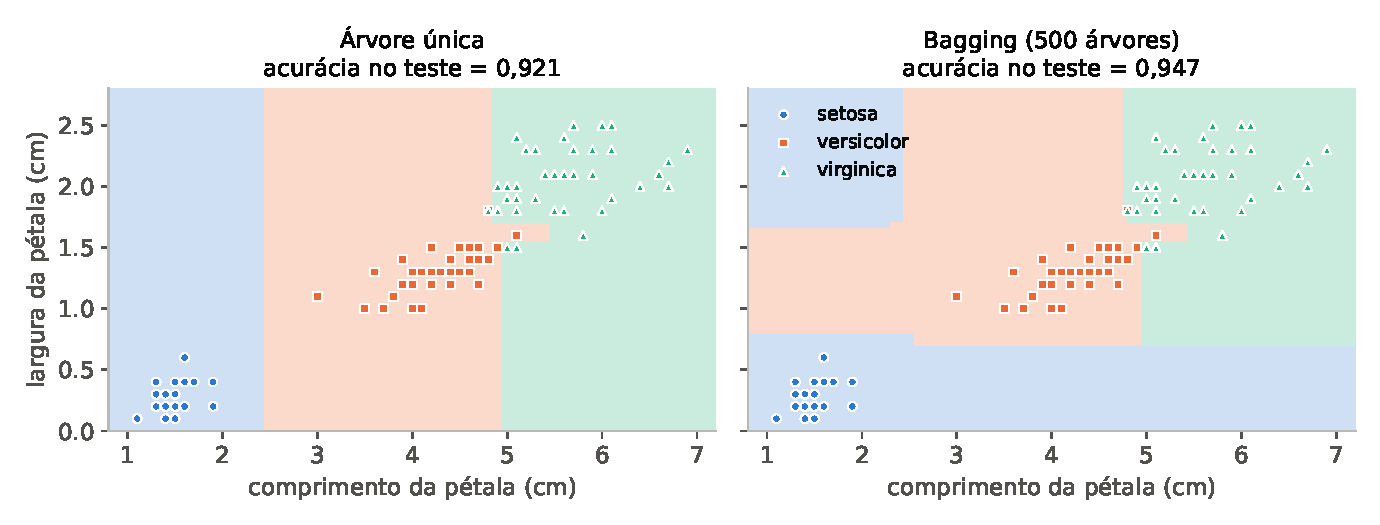
\includegraphics[width=0.84\linewidth]{../python/ensembles/figures/fronteiras_arvore_bagging.pdf}
\vspace{2pt}
\begin{itemize}
  \item Usamos só as duas variáveis da pétala para poder desenhar a fronteira. Treino: $0{,}991$ nos dois; teste: $0{,}921\to0{,}947$ (uma flor).
  \item Na região onde \emph{versicolor} e \emph{virginica} se encontram, cada árvore corta em um lugar ligeiramente diferente; o bagging vota entre esses cortes e a fronteira resultante tem \alert{mais degraus}, mas \alert{não é visivelmente mais suave} que a da árvore única.
\end{itemize}
\end{frame}

\begin{frame}{Quantas árvores? Repetindo 30 divisões}
\begin{columns}[T]
\column{0.56\textwidth}
\centering
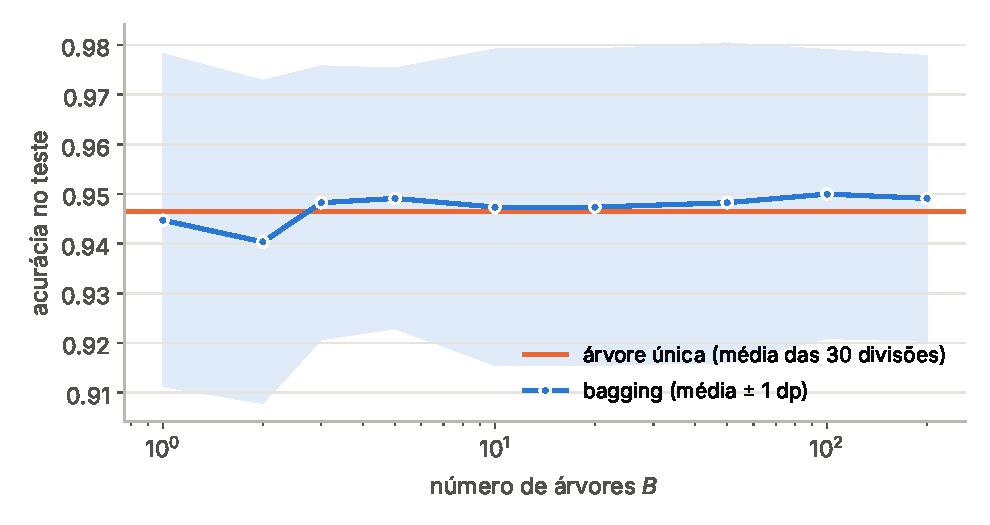
\includegraphics[width=\linewidth]{../python/ensembles/figures/acuracia_vs_B.pdf}
\column{0.42\textwidth}
\small
\begin{itemize}
  \item Árvore única: $0{,}946$ (média).
  \item Bagging: de $0{,}945$ ($B=1$) a $0{,}949$ ($B=200$).
  \item A curva é \alert{praticamente plana}: o ganho ($\approx0{,}3$ p.p.) está muito abaixo do desvio-padrão ($\approx0{,}03$).
  \item Mais árvores não pioram o resultado, mas no Iris também quase não melhoram: há pouca variância a remover.
\end{itemize}
\end{columns}
\end{frame}

\begin{frame}[fragile]{Avaliação \emph{out-of-bag} (OOB)}
Cada árvore não vê $\approx36{,}8\%$ dos pontos de treino; usam-se esses pontos como validação gratuita.

\vspace{4pt}
\lstinputlisting[style=py,firstline=10,lastline=16]{../python/ensembles/05_oob.py}
\vspace{2pt}
{\footnotesize\textbf{Saída}}
\lstinputlisting[style=saida]{../python/ensembles/outputs/05_oob.txt}
\vspace{2pt}
\begin{itemize}
  \item A estimativa OOB ($0{,}946$) fica muito próxima da acurácia de teste ($0{,}947$), sem separar dados de validação.
\end{itemize}
\end{frame}

\begin{frame}{Por que reduz a variância}
Se $\hat f_1,\dots,\hat f_B$ têm variância $\sigma^2$ e correlação par a par $\rho$:
\[
\Var\Bigl(\frac1B\sum_{b=1}^B\hat f_b\Bigr)=\rho\,\sigma^2+\frac{1-\rho}{B}\,\sigma^2 .
\]
\begin{itemize}
  \item Com $\rho=0$ (independentes): variância cai por $B$.
  \item Com $B\to\infty$: sobra $\rho\sigma^2$, o \alert{piso} imposto pela correlação entre as árvores.
  \item O viés praticamente não muda: bagging atua sobre árvores profundas (baixo viés, alta variância).
  \item Árvores de bootstrap são \alert{correlacionadas}: variáveis fortes dominam o topo de todas elas $\Rightarrow$ motivação das florestas.
\end{itemize}
\end{frame}
